
\chapter{SocketCluster}
\label{SocketCluster}
\lhead{Appendix A. \emph{SocketCluster}}
\section{Simple ping-pong exchange}
\textbf{Client code}


This is an example of a WebSocket client code spread on all available cores.
New clients are spawned every \texttt{numberClientsEachSecond}. Thereafter,
every \texttt{intv} each clients sends a ping event cast to a Javascript JSON
object.

\begin{figure}[H]
	\centering
		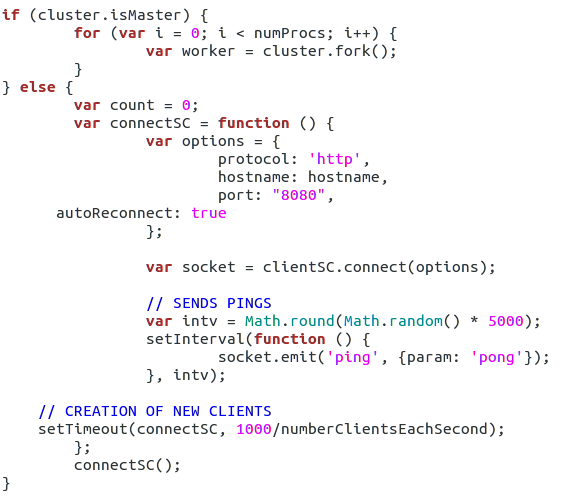
\includegraphics[width=0.7\textwidth]{./Figures/WS_client_simplePing.png}
	\caption[Simple WebSocket client code]{Pings from client}
	\label{fig:WS_client_simplePing}
\end{figure}

To best simulate clients interaction with a websocket server, new sockets are
created at random intervals \texttt{intv = Math.round(Math.random()*5000)}.

\textbf{Server code}

The server listens for pings event and answers back with pongs event. In this
case the pong event is an integer counting the number of pings this particular
worker had during the whole experiment.

\begin{figure}[H]
	\centering
    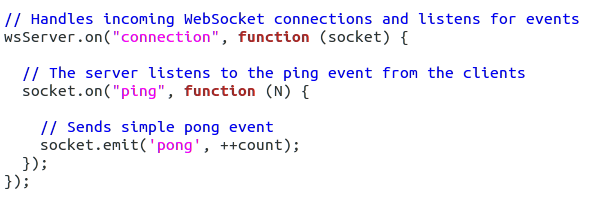
\includegraphics[width=\textwidth]{./Figures/WS_server_simplePong.png}
	\caption[Simple WebSocket server code]{Server answering with pongs}
	\label{fig:WS_server_simplePong}
\end{figure}

\section{File transfer}

\textbf{Client code}

In this example, the goal is to exchange a file using the WebSocket protocol.
For this purpose, the node.js \texttt{delivery} library is used.

New clients are created on the same model as the previous example. Each new
client is stored in the \texttt{clients} array. Each clients are also
periodically sending pings. The only add on is the \texttt{map} function to
enable the each socket to retrieve the document sent by the server. 

\begin{figure}[H] \centering
  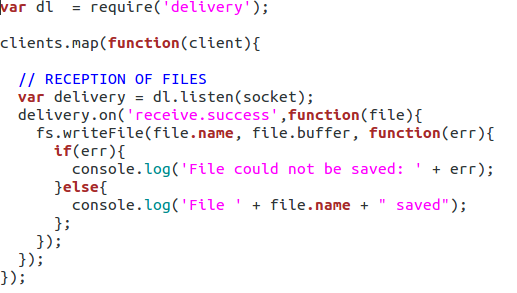
\includegraphics[width=\textwidth]{./Figures/WS_client_delivery.png}
\caption[Client code for file transfers with WebSocket ]{Clients receptionning files} 
\label{fig:WS_client_delivery}
\end{figure}

\textbf{Server code}

The server listens for pings. And sends back a file, \texttt{foo.txt} in this
example.

\begin{figure}[H]
	\centering
    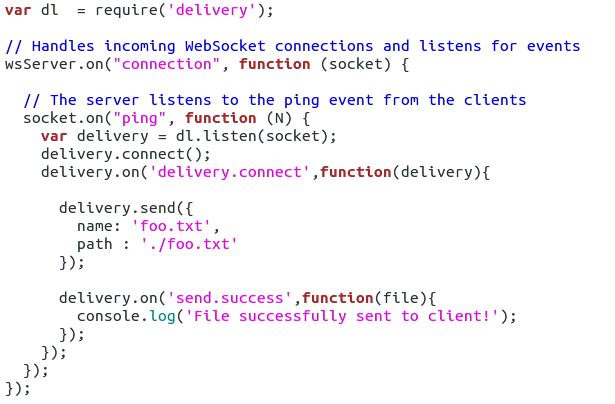
\includegraphics[width=\textwidth]{./Figures/WS_server_delivery.png}
	\caption[Server code for file transfers with Websocket]{Server sending files}
	\label{fig:WS_server_delivery}
\end{figure}

